% !TEX TS-program = pdflatex
% !TeX program = pdflatex
% !TEX encoding = UTF-8
% !TEX spellcheck = fr

\documentclass[xcolor=table]{beamer}


%\usepackage{fullpage}
%\usepackage[left=2.8cm,right=2.2cm,top=2 cm,bottom=2 cm]{geometry}
\setbeamersize{text margin left=10pt,text margin right=10pt}


\usepackage{amsmath,amssymb} 
\usepackage{fontenc}
\usepackage{textcomp}
\usepackage[utf8]{inputenc}
\usepackage{CJKutf8}
\usepackage[french]{babel}
\usepackage{arabtex,acolor}
\usepackage{txfonts}
\usepackage{tipa}
\usepackage[]{graphicx}
\usepackage{multirow}
\usepackage{hyperref}
\usepackage{colortbl}
\usepackage{tabularray}
\usepackage{listingsutf8}
\usepackage{wrapfig}
\usepackage{multicol}
\usepackage[export]{adjustbox} %for images in table, also for frame
\usepackage[many]{tcolorbox}
\usepackage{wasysym}
\usepackage[french,lined]{algorithm2e}
\usepackage{alltt} %verbatim with commands
\usepackage{longtable}
\usepackage{tabu}


\definecolor{lightblue}{HTML}{D0D2FF}
\definecolor{lightyellow}{HTML}{FFFFAA}
\definecolor{darkblue}{HTML}{0000BB}
\definecolor{olivegreen}{HTML}{006600}
\definecolor{darkgreen}{HTML}{008B45} %009B55
\definecolor{violet}{HTML}{6600CC}
%\definecolor{deeppink}{HTML}{FF1493}
\definecolor{orangey}{HTML}{FFBB00}

\usetheme{Warsaw} % Antibes Boadilla Warsaw

\beamertemplatenavigationsymbolsempty


\let\oldcite\cite
\renewcommand{\cite}[1]{{\bfseries\color{orangey}\oldcite{#1}}}

\tcbuselibrary{listings}

\newcommand{\kurl}[1]{{\scriptsize\bfseries\color{orangey}\url{#1}}}


%\renewcommand{\baselinestretch}{1.5}

\def\supit#1{\raisebox{0.8ex}{\small\it #1}\hspace{0.05em}}

\AtBeginSection{%
	\begin{frame}
		\sectionpage
	\end{frame}
}

\newcommand{\rottext}[2]{%
	\rotatebox{90}{%
	\begin{minipage}{#1}%
		\raggedleft#2%
	\end{minipage}%
	}%
}


\institute{ %
Laboratoire de la Communication dans les Systèmes Informatiques (LCSI)

\vspace{6pt}
École  nationale Supérieure d'Informatique (ESI, ex. INI), Alger, Algérie
}
\author[ \textbf{\footnotesize\insertframenumber/\inserttotalframenumber} \hspace*{1cm} ESI - ARIES Abdelkrime (Master 2022/2023)] %
{ARIES Abdelkrime}
%\titlegraphic{
\includegraphics[height=1cm]{../img/esi-logo.png}%\hspace*{4.75cm}~
	
	
	\date{Master 2022/2023} %\today

\titlegraphic{%
	
\includegraphics[height=1cm]{../img/esi-logo.png}%
	\hspace{2cm}
	
\includegraphics[height=1cm]{../img/lcsi-logo.png}%
}


%\setbeamertemplate{headline}{}



\newcommand{\keyword}[1]{\textcolor{red}{\bfseries\itshape #1}}
\newcommand{\expword}[1]{\textcolor{olivegreen}{#1}}
\newcommand{\optword}[1]{\textcolor{violet}{\bfseries #1}}

\makeatletter
\newcommand\mysphere{%
	\parbox[t]{10pt}{\raisebox{0.2pt}{\beamer@usesphere{item projected}{bigsphere}}}}
\makeatother

%\let\oldtabular\tabular
%\let\endoldtabular\endtabular
%\renewenvironment{tabular}{\rowcolors{2}{white}{lightblue}\oldtabular\rowcolor{blue}}{\endoldtabular}


\NoAutoSpacing %french autospacing after ":"

\def\graphpath{}

\newcommand{\changegraphpath}[1]{\def\graphpath{#1}}


\newcommand{\vgraphpage}[2][.84\textheight]{%
%	\begin{center}%
		\includegraphics[height=#1]{\graphpath #2}%
%	\end{center}%
}

\newcommand{\hgraphpage}[2][\textwidth]{%
%	\begin{center}%
		\includegraphics[width=#1]{\graphpath #2}%
%	\end{center}%
}

\newcommand{\graphpage}[2][]{%
	\includegraphics[#1]{\graphpath #2}%
}

\bibliographystyle{apalike}

\newcommand{\insertbibliography}[2]{
	\appendix
	\section*{Bibliographie}
	\nocite{#2}
%	\makeatletter % to change template
%	\setbeamertemplate{headline}[default] % not mandatory, but I though it was better to set it blank
%	\def\beamer@entrycode{\vspace*{-\headheight}} % here is the part we are interested in :)
%	\makeatother
	\begin{multicols*}{2}[\frametitle{\insertsection} \usebeamertemplate*{frametitle}]%\usebeamertemplate*{frametitle}\frametitle{Références}
		\tiny
		\bibliography{#1}
	\end{multicols*}
}

\definecolor{my-grey}{RGB}{233, 233, 233}

\newcommand{\insertlicence}{
	\begin{frame}[plain]
	\frametitle{Licence : CC-BY 4.0}
%	\framesubtitle{Licence: CC-BY-NC 4.0}

	\begin{tcolorbox}[colback=cyan,
		colframe=cyan,  
		arc=0pt,outer arc=0pt,
		valign=top, 
		halign=center,
		width=\textwidth]
		
		
\includegraphics[width=.5cm]{../img/licence/cc_icon_white_x2.png}
		
\includegraphics[width=.5cm]{../img/licence/attribution_icon_white_x2.png}
		
		\color{white}
		\bfseries Attribution 4.0 International (CC BY 4.0) \\
		\tiny \url{https://creativecommons.org/licenses/by/4.0/deed.fr}
		
	\end{tcolorbox}\vspace{-.5cm}
	\begin{tcolorbox}[colback=my-grey,
		colframe=my-grey,  
		center, arc=0pt,outer arc=0pt,
		valign=top, 
		halign=left,
		width=\textwidth]
		
		\tiny
		
		\begin{center}
			\bfseries\Large
			Vous êtes autorisé à :
		\end{center}
		
		\begin{minipage}{0.83\textwidth}
			\begin{itemize}
				\item[] \textbf{Partager} — copier, distribuer et communiquer le matériel par tous moyens et sous tous formats
				\item[] \textbf{Adapter} — remixer, transformer et créer à partir du matériel
				pour toute utilisation, y compris commerciale.
			\end{itemize}
		\end{minipage}
		\begin{minipage}{0.15\textwidth}
			
\includegraphics[width=\textwidth]{../img/licence/FreeCulturalWorks_seal_x2.jpg}
		\end{minipage}
	
		
		\begin{center}
			\bfseries\Large
			Selon les conditions suivantes :
		\end{center}
		
		\begin{itemize}
			\item[] \textbf{Attribution} — Vous devez créditer l'Œuvre, intégrer un lien vers la licence et indiquer si des modifications ont été effectuées à l'Oeuvre. Vous devez indiquer ces informations par tous les moyens raisonnables, sans toutefois suggérer que l'Offrant vous soutient ou soutient la façon dont vous avez utilisé son Oeuvre. 
			\item[] \textbf{Pas de restrictions complémentaires} — Vous n'êtes pas autorisé à appliquer des conditions légales ou des mesures techniques qui restreindraient légalement autrui à utiliser l'Oeuvre dans les conditions décrites par la licence.
		\end{itemize}
		
	\end{tcolorbox}
	
%	\begin{center}
%		\bfseries Attribution 4.0 International (CC BY 4.0)
%		\url{https://creativecommons.org/licenses/by/4.0/deed.fr}
%	\end{center}

%	\tiny
%
%	Vous êtes autorisé à : 
%	\begin{itemize}
%		\item \textbf{Partager} — copier, distribuer et communiquer le matériel par tous moyens et sous tous formats
%		\item \textbf{Adapter} — remixer, transformer et créer à partir du matériel
%	\end{itemize}
%	
%	Selon les conditions suivantes : 
%	\begin{itemize}
%		\item \textbf{Attribution} — Vous devez créditer l'Œuvre, intégrer un lien vers la licence et indiquer si des modifications ont été effectuées à l'Oeuvre. Vous devez indiquer ces informations par tous les moyens raisonnables, sans toutefois suggérer que l'Offrant vous soutient ou soutient la façon dont vous avez utilisé son Oeuvre.
%		\item \textbf{Pas d'Utilisation Commerciale} — Vous n'êtes pas autorisé à faire un usage commercial de cette Oeuvre, tout ou partie du matériel la composant. 
%		\item \textbf{Pas de restrictions complémentaires} — Vous n'êtes pas autorisé à appliquer des conditions légales ou des mesures techniques qui restreindraient légalement autrui à utiliser l'Oeuvre dans les conditions décrites par la licence.
%	\end{itemize}

	\end{frame}
}

\settowidth{\leftmargini}{\usebeamertemplate{itemize item}}
\addtolength{\leftmargini}{\labelsep}

\AtBeginDocument{
	\newcolumntype{L}[2]{>{\vbox to #2\bgroup\vfill\flushleft}p{#1}<{\egroup}} 
	
	\begin{frame}[plain]
		\maketitle
	\end{frame}

	\insertlicence
}


% needs etoolbox; to break links after -
\appto\UrlBreaks{\do\-}


\makeatletter
\newcommand{\xRightarrow}[2][]{\ext@arrow 0359\Rightarrowfill@{#1}{#2}}
\makeatother


\usefonttheme{structurebold}
%\usefonttheme{professionalfonts}

\title[TALN : 05- Analyse syntaxique]%
{Traitement automatique du langage naturel\\Chapitre 05 : Analyse syntaxique} 

\changegraphpath{../img/syntaxe/}

\begin{document}
	
\begin{frame}
\frametitle{Traitement automatique du langage naturel}
\framesubtitle{Analyse syntaxique : Introduction}

\begin{exampleblock}{Exemple d'une phrase en français}
	\begin{center}
		\Large\bfseries
		L'élève a écrit une solution avec son stylo. 
		
		L'élève a écrit une solution avec son explication.
	\end{center}
\end{exampleblock}

\begin{itemize}
	\item Qui a écrit la solution ?
	\item Quel instrument a-t-on utilisé pour l'écriture ?
	\begin{itemize}
		\item Un stylo ? Une explication ?
	\end{itemize}
	\item Est-ce qu'on a écrit d'autres choses en plus de la solution ?
	\begin{itemize}
		\item Un stylo ? Une explication ?
	\end{itemize}
	\item Comment avez-vous déduit ça ?
\end{itemize}

\end{frame}

\begin{frame}
\frametitle{Traitement automatique du langage naturel}
\framesubtitle{Analyse syntaxique : Un peu d'humour}

\begin{center}
	\vgraphpage{humour-parse.jpg}
\end{center}

\end{frame}

\begin{frame}
\frametitle{Traitement automatique du langage naturel}
\framesubtitle{Analyse syntaxique : Plan}

\begin{multicols}{2}
%	\small
\tableofcontents
\end{multicols}
\end{frame}

%===================================================================================
\section{Structures syntaxiques}
%===================================================================================

\begin{frame}
\frametitle{Analyse syntaxique}
\framesubtitle{Structures syntaxiques}

\begin{itemize}
	\item Une phrase peut être bien formée syntaxiquement mais pas sémantiquement 
	\begin{itemize}
		\item Ex. \expword{Les idées vertes et non colorées dorment furieusement.}
	\end{itemize}
	\item Plusieurs théories 
	\begin{itemize}
		\item La grammaire générative et transformationnelle 
		\item La grammaire de dépendance 
		\item La grammaire catégorique
		\item Les grammaires stochastiques
		\item Les approches fonctionnelles de la grammaire
	\end{itemize}
	
\end{itemize}

\end{frame}

%\subsection{Grammaires à contexte libre}

\subsection{Annotation constituante}

\begin{frame}
\frametitle{Analyse syntaxique : Structures syntaxiques}
\framesubtitle{Annotation constituante}

\begin{itemize}
	\item Les mots d'une phrase ont chacun \keyword{une catégorie grammaticale}
	\begin{itemize}
		\item Ex. \expword{Le/DET cours/NOM est/VP intéressant/ADJ}
	\end{itemize}
	\item Un ou plusieurs mots de certaines catégories forment \keyword{un syntagme}
	\begin{itemize}
		\item Ex. \expword{[Le/DET cours/NOM ]\textsubscript{NP} [est/VP intéressant/ADJ VP]\textsubscript{VP}}
	\end{itemize}
\end{itemize}

\begin{center}
	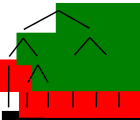
\includegraphics[width=0.4\textwidth]{../img/intro/gram_const.pdf}
\end{center}

\end{frame}

\begin{frame}
\frametitle{Analyse syntaxique : Structures syntaxiques}
\framesubtitle{Annotation constituante : Grammaires à contexte libre (CFG)}

\begin{minipage}{.68\textwidth}
\begin{itemize}
	\item $G <\Sigma, N, P, S>$ est une grammaire.
	\item $\Sigma$ est le vocabulaire : ensemble des symboles terminaux
	\begin{itemize}
		\item \expword{$\Sigma$ = \{le, petit, chat, mange, un, poisson, ...\}}
	\end{itemize}
	\item $N$ est l'ensemble des  variables : symboles non terminaux 
	\begin{itemize}
		\item \expword{$N$ = \{S, NP, VP, DET, N, ADJ, ...\}}
	\end{itemize}
\end{itemize}
\end{minipage}
\begin{minipage}{.3\textwidth}
	\hgraphpage{humour-chomsky.jpg}
\end{minipage}

\begin{itemize}
	\item $S \in N$ est l'axiome.
	\item $P$ est l'ensemble des règles de production.
	\item Les règles sont de la forme $A \rightarrow \beta \text{ avec } A \in N,\, \beta \in (\Sigma \cup N)^*$
	\begin{itemize}
		\item \expword{S \textrightarrow NP VP}
		\item \expword{NP \textrightarrow DET ADJ N \textbar\ DET N}
		\item \expword{VP \textrightarrow V NP}
	\end{itemize}
\end{itemize}

\end{frame}

\begin{frame}
\frametitle{Analyse syntaxique : Structures syntaxiques}
\framesubtitle{Annotation constituante : CFG probabiliste (PCFG)}

\begin{itemize}
	\item $G <\Sigma, N, P, S>$ est une grammaire.
	\item Les règles sont de la forme $A \rightarrow \beta\, [p] \text{ avec } A \in N,\, \beta \in (\Sigma \cup N)^*$
	\item $p$ est la probabilité d'occurrence de la règle
	\item Cette probabilité est estimée à partir d'un corpus annoté (\keyword{TreeBank})
\end{itemize}

\begin{block}{Estimation des probabilité des règles}
	\[
	P(A \rightarrow \beta | A) = \frac{C(A \rightarrow \beta)}{C(A)}
	\]
\end{block}

\end{frame}

\subsection{Annotation fonctionnelle}

\begin{frame}
\frametitle{Analyse syntaxique : Structures syntaxiques}
\framesubtitle{Annotation fonctionnelle}

\begin{itemize}
	\item Un mot ou plus remplissent \keyword{une fonction syntaxique}
	\begin{itemize}
		\item Ex. \expword{sujet, objet, etc.}
	\end{itemize}
	\item Les liens syntaxiques entre les mots d'une phrase sont appelés : \keyword{dépendances}
	\begin{itemize}
		\item Ex. \expword{Le chat mange un poisson} : ici ``chat" est \expword{le sujet} du verbe ``mange"
	\end{itemize}
	\item Une relation de dépendance relie un mot appelé \keyword{tête syntaxique} avec un autre appelé \keyword{dépendant}
\end{itemize}

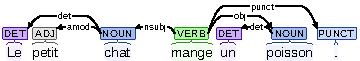
\includegraphics[width=\textwidth]{../img/intro/gram-dep_.pdf}

\end{frame}

\begin{frame}
\frametitle{Analyse syntaxique : Structures syntaxiques}
\framesubtitle{Annotation fonctionnelle : Relations de dépendance}

\begin{table}
	\rowcolors{2}{lightblue}{lightyellow}
	\begin{tabular}{p{.2\textwidth}p{.35\textwidth}p{.35\textwidth}}
		\rowcolor{darkblue}
		\textcolor{white}{Dép. de base} & \textcolor{white}{Description} & \textcolor{white}{Exemple}\\
		nsubj & sujet nominal & Le \underline{people} \textbf{gagne}\\
		obj & objet direct & On \textbf{présente} le \underline{cours}\\
		iobj & objet indirect & Il \underline{m'}\textbf{envoie}\\
		csubj & sujet propositionnel & \underline{Suivre} le cours \textbf{permet} ...\\
		
		\rowcolor{darkblue}
		\textcolor{white}{Dép. des noms} & \textcolor{white}{Description} & \textcolor{white}{Exemple}\\
		amod & modificateur adjectival & La \textbf{fille} \underline{modeste}\\
		det & déterminant & \underline{La} \textbf{fille}\\
		nmod & modificateur nominal & Le \underline{résultat} de la \textbf{course}\\
		nummod & modificateur numérique & J'ai mangé \underline{3} \textbf{bonbons}\\
		
	\end{tabular}
	\caption{Quelques relations de dépendances universelles de Stanford \cite{2014-de-marneffe-al} (\url{https://universaldependencies.org/u/dep/index.html})}
\end{table}

\end{frame}

%===================================================================================
\section{Analyse des constituants}
%===================================================================================

\begin{frame}
\frametitle{Analyse syntaxique}
\framesubtitle{Analyse des constituants}

\begin{itemize}
	\item La grammaire à contexte libre : le système formel le plus utilisé pour modéliser la structure constituante
	\item Analyse 
	\begin{itemize}
		\item \optword{ascendante} : à partir des mots de la phrase, on essaye de trouver les catégories grammaticales. Ensuite, les syntagmes qui génèrent une combinaison des catégories et des syntagmes. On fait ça jusqu'à arriver à \keyword{S}
		\item \optword{descendante} : à partir de \keyword{S}, on cherche les règles qui génèrent la phrase. Ceci en se basant sur des mots pour guider la génération.
	\end{itemize}
\end{itemize}

\begin{center}
	\begin{tabular}{|p{.25\textwidth}|p{.3\textwidth}|p{.3\textwidth}|}
	\hline
	& Classique & Statistique \\
	\hline
	Ascendante & \optword{CKY}, LR & \optword{CKY probabiliste}\\
	\hline
	Descendante & Early, LL, Descente récursive  & \\
	\hline
\end{tabular}
\end{center}

\end{frame}

\subsection{Algorithme CKY}

\begin{frame}
\frametitle{Analyse syntaxique : Analyse des constituants}
\framesubtitle{Algorithme CKY}

\begin{itemize}
	\item Algorithme de \keyword{Cocke-Kasami-Younger}
	\item Analyse ascendante
	\item Prérequis : Forme normale de Chomsky
\end{itemize}

\begin{definition}[FNC : Forme normale de Chomsky]
	\[
	A \rightarrow  B C \text{ où } A, B, C \in N
	\]
	
	\[
	A \rightarrow w \text{ où } w \in \Sigma
	\]
\end{definition}

\end{frame}

\begin{frame}
\frametitle{Analyse syntaxique : Analyse des constituants}
\framesubtitle{Algorithme CKY : Reconnaissance d'une phrase}

\vspace{-6pt}
\begin{block}{CKY : Reconnaissance d'une phrase}
	\scriptsize\vspace{-3pt}
	\begin{algorithm}[H]
		\Donnees{une grammaire $G <\Sigma, N, P, S>$ en FNC; une phrase $w = w_1 \ldots w_n$}
		\Res{$T[n, n]$}
		
		\Pour{$ i = 1 \ldots n$}{ %\tcc*{Initialiser le diagonal}
			$T[i, i] \leftarrow \{ (A, 0, 0, 0) / (A \rightarrow w_i) \in P \} $\;
		}
		
		\Pour{$ i = (n-1) \ldots 1$ }{
			\Pour{$ j = (i+1) \ldots n $}{
				\Pour{$ k = i \ldots (j-1) $}{
					\PourTous{$A$ tel que $(A \rightarrow B C) \in P $ et $B \in T[i, k]$ et $C \in T[k+1, j]$}{
						$iB \leftarrow index(B, T[i, k])$ ;
						$iC \leftarrow index(C, T[k+1, j])$ \;
						$T[i, j] \leftarrow T[i, j] \cup \{(A, k, iB, iC)\}$ \;
					}
				}
			}
		}
		
		\Si{$``S" \notin T[1, n] $} {
			Erreur ``La phrase n'a pas été reconnue"\;
		}
		\vspace{-3pt}
	\end{algorithm}
\end{block}

\end{frame}

\begin{frame}
\frametitle{Analyse syntaxique : Analyse des constituants}
\framesubtitle{Algorithme CKY : Construction de l'arbre}

\vspace{-6pt}
\begin{block}{CKY : Construction de l'arbre}
	\scriptsize\vspace{-3pt}
	\begin{algorithm}[H]
		\SetKwFunction{FConst}{Construire}
		\SetKwProg{Fn}{Fonction}{\\Début}{Fin}
		
		\Donnees{$T[n, n]$}
		\Res{Racine de l'arbre syntaxique : $r \leftarrow \varnothing$}
		
		\Si{$``S" \in T[1, n] $} {
			$r \leftarrow $ \FConst{$1, n, index(``S", T[1, n])$}\;
		}
		
		\Fn{\FConst{$i, j, pos$}}{
			$ (A, k, iB, iC) \leftarrow T[i, j][pos] $\;
			Créer un nouveau nœud : nœud\;
			nœud.valeur $\leftarrow  A$ \;
			\Si{$k>0$}{
				nœud.gauche $\leftarrow$ \FConst{$i, k, iB$}\;
				nœud.droit $\leftarrow$ \FConst{$k+1, j, iC$}\;
			}
			\Retour nœud\;
		}
		
		
%		\vspace{-3pt}
	\end{algorithm}
\end{block}

\end{frame}

\begin{frame}
\frametitle{Analyse syntaxique : Analyse des constituants}
\framesubtitle{Algorithme CKY : Exercice}

\vspace{-6pt}
\begin{exampleblock}{Exemple d'une grammaire}
	\begin{itemize}
		\item S \textrightarrow\ NP VP 
		\item S \textrightarrow\ VP 
		\item VP \textrightarrow V NP
		\item NP \textrightarrow\ DET ADJ N \textbar\ DET N \textbar\ PRON 
		\item PRON \textrightarrow\ je \textbar\ tu \textbar\ il \textbar\ elle
		\item V \textrightarrow\ forme \textbar\ veut \textbar\ mange 
		\item DET \textrightarrow\ un \textbar\ une \textbar\ la \textbar\ le
		\item ADJ \textrightarrow\ petite \textbar\ grand \textbar\ bleu 
		\item N \textrightarrow\ petite \textbar\ forme \textbar\ phrase \textbar\ chat \textbar\ poisson
	\end{itemize}
\end{exampleblock}\vspace{-6pt}

\begin{itemize}
	\item Analyser la phrase suivante en utilisant CKY 
	\item \expword{la petite forme une petite phrase}
\end{itemize}

\end{frame}

\begin{frame}
\frametitle{Analyse syntaxique : Analyse des constituants}
\framesubtitle{Algorithme CKY : Remarques}

\begin{minipage}{.53\textwidth}
\begin{itemize}
	\item L'arbre syntaxique résultante est binaire. Mais, dans la réalité elle doit suivre la grammaire conçue par les syntacticiens
	\begin{itemize}
		\item Ajouter une étape de post-traitement pour récupérer l'arbre originale
		\item Laisser les productions unitaires et modifier l'algorithme CKY afin de les accepter
	\end{itemize}
	\item Problème d'ambigüité syntaxique 
	\begin{itemize}
		\item Ex. \expword{Je mange du riz avec une fourchette.} et \expword{Je mange du riz avec de la viande.}
%		\item 
	\end{itemize}
\end{itemize}
\end{minipage}
\begin{minipage}{.45\textwidth}
	\hgraphpage{humour-ambiguity.jpg}
\end{minipage}

\end{frame}

\subsection{Algorithme CKY probabiliste}

\begin{frame}
\frametitle{Analyse syntaxique : Analyse des constituants}
\framesubtitle{Algorithme CKY probabiliste}

\begin{itemize}
	\item $G<\Sigma, N, P, S>$ est une grammaire probabiliste
	\item Les nouvelles règles créées par transformation en FNC ont une probabilité égale à $1$
	\item $w = w_1 \ldots w_n$ est un mot à analyser 
	\item $T$ est un arbre syntaxique 
	\item $P(T, w) = \prod\limits_{(A_i \rightarrow \beta_i) \in T} P(A_i \rightarrow \beta_i)$ est la probabilité d'un arbre syntaxique étant donné le mot analysé $w$
	\item $\hat{T}(w) = \arg\max\limits_{T(w)} P(T, w) $ est l'arbre syntaxique le plus adéquat pour analyser le mot $w$
\end{itemize}

\end{frame}

\begin{frame}
\frametitle{Analyse syntaxique : Analyse des constituants}
\framesubtitle{Algorithme CKY probabiliste : Reconnaissance d'une phrase}

\vspace{-6pt}
\begin{block}{CKY probabiliste : Reconnaissance d'une phrase}
	\scriptsize\vspace{-3pt}
	\begin{algorithm}[H]
		\Donnees{une grammaire $G <\Sigma, N, P, S>$ en FNC; une phrase $w = w_1 \ldots w_n$}
		\Res{$T[n, n, |N|]$}
		
		\Pour{$ i = 1 \ldots n$}{ %\tcc*{Initialiser le diagonal}
			$T[i, i, A] \leftarrow \{ (P(A \rightarrow w_i), 0, A, A) / (A \rightarrow w_i) \in P \} $\;
		}
		
		\Pour{$ i = (n-1) \ldots 1$ }{
			\Pour{$ j = (i+1) \ldots n $}{
				\Pour{$ k = i \ldots (j-1) $}{
					\PourTous{$A$ tel que $(A \rightarrow B C) \in P $ et $T[i, k, B] > 0$ et $T[k+1, j, C] > 0$}{
						$p \rightarrow P(A \rightarrow B C) * T[i, k, B][1] * T[k+1, j, C][1]$\;
						\Si{$p > T[i, j, A][1]$}{
							$T[i, j, A] \leftarrow (p, k, B, C)$ \;
						}
					}
				}
			}
		}
		
		\Si{$T[1, n, S] = 0 $} {
			Erreur ``La phrase n'a pas été reconnue"\;
		}
		\vspace{-3pt}
	\end{algorithm}
\end{block}

\end{frame}


%===================================================================================
\section{Analyse des dépendances}
%===================================================================================

\begin{frame}
\frametitle{Analyse syntaxique}
\framesubtitle{Analyse des dépendances}

\begin{minipage}{.6\textwidth}
\begin{itemize}
	\item \optword{Analyse basée sur les transitions} 
	\begin{itemize}
		\item \textbf{Configuration} :  $C = (\sigma, \beta, A)$ où $\sigma$ est une pile, $\beta$ est le tampon (buffer) d'entrée et $A$ est la liste des arcs créés
		\item $C_{initiale} = ([ROOT], w, \emptyset)$
		\item $C_{finale} = ([ROOT], \varnothing, A)$
%		\item Un ensemble d'actions possibles
	\end{itemize}
\end{itemize}
\end{minipage}
\begin{minipage}{.38\textwidth}
	\hgraphpage{transitions.pdf}
\end{minipage}

%
\vfill

\begin{minipage}{.6\textwidth}
	\begin{itemize}
		\item \optword{Analyse basée sur les graphes}
		\begin{itemize}
			\item \textbf{Graphe} : $G = (V, E)$ où $V$ est l'ensemble de nœuds (mots) et $E$ l'ensemble d'arcs (relations de dépendance)
			\item \textbf{Résultat} : $T = (V, F)$ un sous-graphe de $G$ représentant les relations de dépendance
		\end{itemize}
	\end{itemize}
\end{minipage}
\begin{minipage}{.38\textwidth}
	\hgraphpage{graphe.pdf}
\end{minipage}

\end{frame}

\subsection{Par transition}

\begin{frame}
\frametitle{Analyse syntaxique : Analyse des dépendances}
\framesubtitle{Par transition}

\begin{minipage}{.6\textwidth}
	\begin{itemize}
		\item \textbf{Configuration} :  $C = (\sigma, \beta, A)$
		\begin{itemize}
			\item $\sigma$ est une pile
			\item $\beta$ est le tampon (buffer) d'entrée
			\item $A$ est la liste des arcs créés (dépendances)
			\item $C_{initiale} = ([ROOT], w, \emptyset)$
			\item $C_{finale} = ([ROOT], \varnothing, A)$
		\end{itemize}
	\end{itemize}
\end{minipage}
\begin{minipage}{.38\textwidth}
	\hgraphpage{transitions.pdf}
\end{minipage}

\begin{itemize}
	\item \textbf{Transition} : passer d'un état vers un autre en utilisant des actions sur
	\begin{itemize}
		\item $\sigma$ : empiler ou dépiler un mot
		\item $\beta$ : retirer un mot ou ajouter un au début
		\item $A$ : ajouter une dépendance entre 2 mots
	\end{itemize}
	\item \textbf{Oracle} : un système qui décide la transition suivante
\end{itemize}

\end{frame}

\begin{frame}
\frametitle{Analyse syntaxique : Analyse des dépendances}
\framesubtitle{Par transition : Algorithme d'analyse}

\begin{itemize}
	\item Le système ``$Oracle$" choisit une transition ``$t$"
	\item La fonction ``$Appliquer$" exécute ``$t$" sur la configuration
\end{itemize}

\begin{block}{Analyse des dépendances par transitions}
	\begin{algorithm}[H]
		\Donnees{Le mot à analyser $w= w_1 w_2 \ldots w_n$}
		\Res{Liste des dépendances $A$}
		
		$C \leftarrow (\sigma=[ROOT], \beta = w, A = \emptyset)$\;
		
		
		\Tq{$\sigma \ne [ROOT]$ OU $\beta \ne \varnothing$}{
			$t \leftarrow Oracle(C)$\;
			$C \leftarrow Appliquer(C, t)$\;
		}
	
		\Retour $A$ \;
	\end{algorithm}
\end{block}

\end{frame}

\begin{frame}
\frametitle{Analyse syntaxique : Analyse des dépendances}
\framesubtitle{Par transition : Système Oracle (entraînement)}

\begin{itemize}
	\item Le système Oracle apprend à inférer la transition $\hat{t}$ étant donné
	\begin{itemize}
		\item la configuration actuelle $ C = (\sigma, \beta, A) $
		\item l'ensemble $T$ des transactions possibles
		\item une fonction $\Psi$ qui calcule un score en utilisant sur des caractéristiques basées sur la configuration 
		\item un texte annoté (TreeBank)
	\end{itemize}
	\[ \hat{t} = \arg\max\limits_{t \in T} \Psi (t, C, w; \theta) \]
	
	\item Le texte annoté doit être transformé à une séquence de transactions
	\item Pour entraîner l'Oracle, on utilise l'algorithme d'analyse 
	\item La fonction $\Psi$ peut être MaxEnt (le plus utilisé), SVM ou les réseaux de neurones
\end{itemize}

\end{frame}

\begin{frame}
\frametitle{Analyse syntaxique : Analyse des dépendances}
\framesubtitle{Par transition : Système Oracle (caractéristiques)}

\begin{itemize}
	\item \textbf{La pile $\sigma$}
	\begin{itemize}
		\item Le mot dans le sommet de la pile
		\item La catégorie grammaticale de ce mot
	\end{itemize}

	\item \textbf{Le tampon d'entrée $\beta$}
	\begin{itemize}
		\item Les trois premiers mots
		\item Leurs catégories grammaticales
	\end{itemize}

	\item \textbf{La liste des dépendances $A$}
	\begin{itemize}
		\item Les dépendances qui ont été estimées
	\end{itemize}

	\item \textbf{La phrase analysée $w$}
	\begin{itemize}
		\item La distance entre le mot du sommet de la pile et le premier mot dans le tampon (nombre des mots entre eux dans la phrase $w$)
	\end{itemize}

\end{itemize}

\end{frame}

\begin{frame}
\frametitle{Analyse syntaxique : Analyse des dépendances}
\framesubtitle{Par transition : Arc-standard (transitions possibles)}

\begin{itemize}
	\item \optword{SHIFT} : Déplacer le premier élément dans le tampon vers la pile 
	\[ (\sigma, w_i|\beta, A) \Rightarrow  (\sigma|w_i, \beta, A) \]
	
	\item \optword{ARC-LEFT} : Établir un arc du premier élément dans le tampon vers le sommet de la pile
	\[ (\sigma|w_i, w_j|\beta, A) \Rightarrow  (\sigma, w_j|\beta, A \cup \{w_j \rightarrow w_i \}) \] 
	
	\item \optword{ARC-RIGHT} : Établir un arc du sommet de la pile vers le premier élément dans le tampon
	\[ (\sigma|w_i, w_j|\beta, A) \Rightarrow  (\sigma, w_i|\beta, A \cup \{w_i \rightarrow w_j \}) \] 
\end{itemize}

\end{frame}


\begin{frame}
\frametitle{Analyse syntaxique : Analyse des dépendances}
\framesubtitle{Par transition : Arc-standard (exemple)}

\begin{figure}
	\hgraphpage{exp-arc-std_.pdf}
	\caption{Exemple de dérivations non étiquetées de la phrase ``\expword{they like bagels with lox}" en utilisant Arc-standard \cite{2018-eisenstein}}
\end{figure}

\end{frame}


\begin{frame}
\frametitle{Analyse syntaxique : Analyse des dépendances}
\framesubtitle{Par transition : Arc-Eager (transitions possibles)}

\begin{itemize}
	\item \optword{SHIFT} est le même que ``Arc-standard"
	
	\item \optword{ARC-LEFT} : Établir un arc du premier élément dans le tampon vers le sommet de la pile
	\[ (\sigma|w_i, w_j|\beta, A) \xRightarrow{\forall w_k (w_k \rightarrow w_i) \notin A}  (\sigma, w_j|\beta, A \cup \{w_j \rightarrow w_i \}) \] 
	
	\item \optword{ARC-RIGHT} : Établir un arc du sommet de la pile vers le premier élément dans le tampon
	\[ (\sigma|w_i, w_j|\beta, A) \Rightarrow  (\sigma|w_i w_j, \beta, A \cup \{w_i \rightarrow w_j \}) \] 
	
	\item \optword{REDUCE} : Dépiler un mot s'il a déjà un parent
	\[ (\sigma|w_i, \beta, A) \xRightarrow{\exists w_k (w_k \rightarrow w_i) \in A} (\sigma, \beta, A) \] 
%	\[ (\sigma|w_i, \beta, \mathcal{A}) \overset{\exists w_k (w_k \rightarrow w_i) \in \mathcal{A}}{\Longrightarrow} (\sigma, \beta, \mathcal{A}) \] 
\end{itemize}

\end{frame}

\begin{frame}
\frametitle{Analyse syntaxique : Analyse des dépendances}
\framesubtitle{Par transition : Arc-Eager (exemple)}

\begin{figure}
	\hgraphpage{exp-arc-eager_.pdf}
	\caption{Exemple de dérivations non étiquetées de la phrase ``\expword{they like bagels with lox}" en utilisant Arc-eager \cite{2018-eisenstein}}
\end{figure}

\end{frame}

\subsection{Par graphe}

%\begin{frame}
%\frametitle{Analyse syntaxique : Analyse des dépendances}
%\framesubtitle{Par graphe}
%
%\begin{minipage}{.6\textwidth}
%	\begin{itemize}
%		\item Analyse basée sur les graphes
%		\begin{itemize}
%			\item Graphe : $G = (V, E)$ où $V$ est l'ensemble de nœuds (mots) et $E$ l'ensemble d'arcs (relations de dépendance)
%			\item Résultat : $T = (V, F)$ un sous-graphe de $G$ représentant les relations de dépendance
%		\end{itemize}
%	\end{itemize}
%\end{minipage}
%\begin{minipage}{.38\textwidth}
%	\hgraphpage{graphe.pdf}
%\end{minipage}
%
%\begin{itemize}
%	\item $\Psi$ est une fonction de score, $ \mathcal{T}(G) $ est l'espace des arbres de dépendance possibles sur $G$
%	\[ \hat{T} = \arg\max\limits_{T \in \mathcal{T}(G)} \Psi(T, w; \theta) \]
%	\item Ce score est calculé en se basant sur le score de chaque arc $\psi$
%	\[ \Psi(T, w; \theta) = \sum_{e \in F / T = (V, F)} \psi(e, w; \theta) \]
%\end{itemize}
%
%\end{frame}

\begin{frame}
\frametitle{Analyse syntaxique : Analyse des dépendances}
\framesubtitle{Par graphe}

\begin{minipage}{.6\textwidth}
	\begin{itemize}
		\item Analyse basée sur les graphes
		\begin{itemize}
			\item \textbf{Graphe} : $G = (V, E)$ où $V$ est l'ensemble de nœuds (mots) et $E$ l'ensemble d'arcs (relations de dépendance)
			\item \textbf{Résultat} : $T = (V, F)$ un sous-graphe de $G$ représentant les relations de dépendance
		\end{itemize}
	\end{itemize}
\end{minipage}
\begin{minipage}{.38\textwidth}
	\hgraphpage{graphe.pdf}
\end{minipage}

\begin{itemize}
	\item $\Psi$ est une fonction de score, $ \mathcal{T}(G) $ est l'espace des arbres de dépendance possibles sur $G$
	\[ \hat{T} = \arg\max\limits_{T \in \mathcal{T}(G)} \Psi(T, w; \theta) \]
	\item Ce score est calculé en se basant sur le score de chaque arc $\psi$
	\[ \Psi(T, w; \theta) = \sum_{e \in F / T = (V, F)} \psi(e, w; \theta) \]
\end{itemize}

\end{frame}

\begin{frame}
\frametitle{Analyse syntaxique : Analyse des dépendances}
\framesubtitle{Par graphe : Score et entraînement}

\begin{itemize}
	\item Le score d'un arc dépend de certaines caractéristiques (d'ordre $K$)
	\[ \psi(e, w; \theta) = \sum_{k = 1}^{K} \theta_k f_k(e, w)  \]
	
	\item Quelques caractéristiques 
	\begin{itemize}
		\item Le mot de l'entête, sa catégorie grammaticale, son lemme, ses préfixes et suffixes
		\item La direction de l'arc
		\item La distance entre l'entête et le dépendant
		\item \ldots
	\end{itemize}
	
\end{itemize}

\end{frame}

\begin{frame}
\frametitle{Analyse syntaxique : Analyse des dépendances}
\framesubtitle{Par graphe : Analyse de Chu-Liu/Edmonds}

\begin{itemize}
	\item On ajoute un nœud (ROOT) avec des arcs vers tous le reste des nœuds 
	\item Les arcs sont pondérés où le poids d'un arc $e$ est $G.p(e)$
	\item On construit un \keyword{Arbre couvrant} de poids maximal
	\item \keyword{Arbre couvrant} : Un sous-graphe acyclique maximal où tous les nœuds sont connectés et il n'y a pas plus qu'un arc entrant vers un nœud
	\item \optword{Contracter} : une fonction qui fusionne deux nœuds $u$ et $v$ composant un cycle $C$
	\begin{itemize}
		\item $\forall e = (u', v) \in E : G.p(e) \leftarrow G.p(e) - G.p((u, v)) $
		\item $\forall e = (v', u) \in E : G.p(e) \leftarrow G.p(e) - G.p((v, u)) $
	\end{itemize}
	\item \optword{Etendre} : une fonction qui désassemble les deux nœuds $u$ et $v$ d'un cycle $C$. L'arc qui enfreint la condition ``\textit{pas de deux arcs entrants}" est supprimé
\end{itemize}
 
\end{frame}

\begin{frame}
\frametitle{Analyse syntaxique : Analyse des dépendances}
\framesubtitle{Par graphe : Analyse de Chu-Liu-Edmonds (Algorithme)}

\vspace{-3pt}
\begin{block}{Analyse de Chu-Liu-Edmonds : Arbre couvrant de poids maximal}
	\scriptsize\vspace{-6pt}
	\begin{algorithm}[H]
		\Donnees{un graphe pondéré $G = (V, E)$, $ ROOT $}
		\Res{un arbre couvrant $T = (V, F)$}
		
		\SetKwFunction{ACM}{ArbreCouvrantMax}
		\SetKwProg{Fn}{Fonction}{}{Fin Fonction} 
		
		\Fn{\ACM{$G, ROOT$}}{
		
		$F \leftarrow \emptyset$\;
		
		\PourTous{$ v \in V$}{ 
			$meilleurInArc \leftarrow \arg\max_{e = (u, v) \in E} G.p(e) $;
			$F \leftarrow F \cup meilleurInArc$\;
			\PourTous{$e = (u, v) \in E$}{ 
				$ G.p(e) \leftarrow G.p(e) - G.p(meilleurInArc) $\;
			}
			\eSi{$T = (V, F)$ est un arbre couvrant}{
				\Retour $T$ \;
			}{
				$C \leftarrow$ un cycle de $F$;
				$G' \leftarrow Contracter(G, C)$\;
				$T' \leftarrow ArbreCouvrantMax(G', ROOT)$;
				$T \leftarrow Etendre(T', C)$\;
				\Retour $T$ \;
			}
		}
	
		}
		\vspace{-3pt}
	\end{algorithm}\vspace{-3pt}
\end{block}

\end{frame}

\begin{frame}
\frametitle{Analyse syntaxique : Analyse des dépendances}
\framesubtitle{Par graphe : Analyse de Chu-Liu-Edmonds (Exercice)}

\begin{figure}
	\centering
	\hgraphpage[.8\textwidth]{exp-graphe_.pdf}
	\caption{Exemple d'un graphe de la phrase ``Book a flight" \cite{2019-jurafsky-martin}}
\end{figure}

\end{frame}


\insertbibliography{TALN05}{*}

\end{document}

